\documentclass[11pt]{article}

\usepackage[margin=1in]{geometry}
\usepackage{graphicx}
\usepackage{amsmath,amssymb}
\usepackage{booktabs}
\usepackage{hyperref}
\usepackage{caption}
\usepackage{subcaption}
\usepackage{enumitem}
\usepackage{xcolor}
\usepackage{float}

\title{Certified and Empirical Uncertainty Quantification\\in Matmul-Free Language Models via Bound Propagation}
\author{%
    \texttt{steven202} \\
    DATA 691 -- Trustworthy AI -- Final Project
}
\date{May 2026}

\begin{document}
\maketitle

\begin{abstract}
Quantifying uncertainty in large language model (LLM) outputs is essential for trustworthy deployment. Formal verification methods such as Interval Bound Propagation (IBP) and CROWN provide \emph{certified} guarantees that model predictions stay within provable bounds under input perturbations. We apply these techniques to MMfreeLM (370M--2.7B parameters), a family of matmul-free recurrent language models that replace dense matrix multiplications with ternary-weight additions. We perturb continuous token embeddings within an $L_\infty$ ball and propagate bounds through the network. We find that certified IBP bounds explode within a single layer---not because of network depth or the ternary weight structure, but because RMSNorm (data-dependent \emph{division}) and multiplicative gating in the recurrence are fundamentally incompatible with interval arithmetic. Sampling-based methods yield finite uncertainty estimates. Comparing MMfreeLM-370M against a standard Transformer baseline (GPT-2 Medium, 355M), we find that the matmul-free architecture exhibits comparable perturbation sensitivity. We analyze how CROWN and IBP-CROWN, which back-propagate linear bounds rather than forward intervals, could address the RMSNorm bottleneck and enable practical certified UQ for recurrent LLMs.
\end{abstract}

\section{Introduction}

Large language models are increasingly deployed in high-stakes applications, yet their robustness to small input variations remains poorly understood. A model that produces radically different outputs under imperceptible input changes is untrustworthy. Uncertainty quantification (UQ)---measuring output variability under bounded perturbations---is therefore central to trustworthy AI.

Two paradigms exist for UQ under perturbations:
\begin{enumerate}[label=(\roman*)]
    \item \textbf{Sampling-based (non-certified)}: estimate output variation by evaluating the model on perturbed inputs. Fast and practical, but provide no formal guarantee that all possible perturbations have been covered.
    \item \textbf{Certified methods}: interval bound propagation (IBP) and CROWN provide provable upper and lower bounds on outputs over \emph{all} perturbations within a set. Sound, but may produce loose or vacuous bounds for deep networks.
\end{enumerate}

We apply both paradigms to MMfreeLM~\cite{zhu2024scalable}, a family of efficient recurrent LMs that replace dense matrix multiplications with ternary weight quantization (BitLinear) and self-attention with a gated linear recurrence (MLGRU). Despite the ``matmul-free'' branding, these models are \textbf{not} purely additive: they contain RMSNorm (division by a data-dependent norm), sigmoid/SwiGLU nonlinearities, and multiplicative gating in the recurrence---all of which challenge certified bound propagation.

We study three model sizes (370M, 1.3B, 2.7B parameters) and a standard Transformer baseline (GPT-2 Medium, 355M), asking: \emph{How much does the output distribution shift when token embeddings are perturbed within an $L_\infty$ ball of radius $\varepsilon$?}

Our contributions are: (1) a diagnosis of \emph{why} IBP fails for recurrent LLMs, identifying RMSNorm as the bottleneck; (2) empirical UQ results across model sizes and architectures; (3) a baseline comparison showing that matmul-free and standard Transformers exhibit comparable perturbation sensitivity; and (4) an analysis of how CROWN and IBP-CROWN could address these limitations.

\section{Methods}

\subsection{Problem Formulation}

Let $f: \mathbb{R}^{L \times d} \to \mathbb{R}^{L \times V}$ be a language model mapping $L$ token embeddings to logits over vocabulary $V$. For nominal embedding $\mathbf{x}$, define the $L_\infty$ perturbation ball:
\begin{equation}
\mathcal{B}_\varepsilon(\mathbf{x}) = \{\mathbf{x}' : \|\mathbf{x}' - \mathbf{x}\|_\infty \leq \varepsilon\}
\end{equation}
We seek bounds $f^L, f^U$ such that $f^L \leq f(\mathbf{x}') \leq f^U$ (element-wise) for all $\mathbf{x}' \in \mathcal{B}_\varepsilon(\mathbf{x})$. The bound width $f^U - f^L$ quantifies output uncertainty.

\subsection{Interval Bound Propagation (Certified)}

IBP~\cite{gowal2018effectiveness} propagates interval tensors $[\mathbf{h}^L, \mathbf{h}^U]$ layer-by-layer. For an affine layer $\mathbf{h} \mapsto \mathbf{W}\mathbf{h} + \mathbf{b}$:
\begin{equation}
\mathbf{h}'^L = \mathbf{W}\boldsymbol{\mu} - |\mathbf{W}|\mathbf{r} + \mathbf{b}, \quad
\mathbf{h}'^U = \mathbf{W}\boldsymbol{\mu} + |\mathbf{W}|\mathbf{r} + \mathbf{b}
\end{equation}
with $\boldsymbol{\mu} = (\mathbf{h}^U + \mathbf{h}^L)/2$, $\mathbf{r} = (\mathbf{h}^U - \mathbf{h}^L)/2$. For monotonic activations $\sigma$: $\mathbf{h}'^L = \sigma(\mathbf{h}^L)$, $\mathbf{h}'^U = \sigma(\mathbf{h}^U)$. We implement IBP following the CROWN-IBP pattern~\cite{zhang2019towards} for BitLinear (ternary $\{-1,0,+1\}$ weights, treated as standard linear), sigmoid, SwiGLU, gated recurrence, and RMSNorm.

\subsection{Sampling-Based Bounds (Non-Certified)}

As practical alternatives that work for \emph{any} model architecture without requiring layer-specific bound implementations, we use:

\textbf{Two-pass corner evaluation}: Run the model on the two extreme embeddings $\mathbf{x} - \varepsilon$ and $\mathbf{x} + \varepsilon$, then take element-wise $\min$/$\max$ of the outputs. Fast (2 forward passes) but not certified---for non-monotonic models, the output extremum need not occur at an input extremum.

\textbf{Monte Carlo (MC) sampling} ($K{=}50$): Sample $K$ random points uniformly from $\mathcal{B}_\varepsilon(\mathbf{x})$, compute model outputs, and take element-wise extrema:
\begin{equation}
f^L \approx \min_{k=1}^K f(\mathbf{x}^{(k)}), \quad f^U \approx \max_{k=1}^K f(\mathbf{x}^{(k)})
\end{equation}
These are \textbf{not} certified but approach the true empirical bounds as $K \to \infty$, and are tighter than the two-pass heuristic.

\subsection{Metrics}

\begin{itemize}[nosep]
    \item \textbf{Mean bound width}: $\frac{1}{LV}\sum_{i,j} |f^U_{ij} - f^L_{ij}|$
    \item \textbf{Top-1 stability}: fraction of positions where $\arg\max f^L = \arg\max f^U$
    \item \textbf{Certified margin}: $f^L_c - \max_{j \neq c} f^U_j$ for predicted class $c$
\end{itemize}

\section{Experimental Setup}

\textbf{Models}: MMfreeLM-370M (24 layers, $d{=}1024$), MMfreeLM-1.3B (24 layers, $d{=}2048$), MMfreeLM-2.7B (32 layers, $d{=}2560$) from HuggingFace.\footnote{\texttt{ridger/MMfreeLM-*}} Baseline: GPT-2 Medium (24 layers, $d{=}1024$, 355M params, \texttt{openai-community/gpt2-medium}), a standard Transformer decoder with dense linear layers, multi-head self-attention, and GELU activations.

\textbf{Prompts}: Five prompts spanning factual knowledge, sentence completion, and open-ended generation (max 32 tokens).

\textbf{Perturbation}: $L_\infty$ noise on continuous token embeddings at $\varepsilon \in \{0.001, 0.005, 0.01, 0.05, 0.1\}$ ($\sim$0.1\%--10\% of typical embedding magnitude).

\textbf{Implementation}: Custom bound propagation in PyTorch 2.2, single NVIDIA GPU. Code available at \url{https://github.com/steven202/DATA691_TrustworthyAI}.

\section{Results}

\subsection{Why IBP Explodes: Division, Not Addition, Is the Bottleneck}

\label{sec:rmsnorm}

A key finding is \emph{why} IBP fails despite MMfreeLM's simplified arithmetic. The model replaces MatMul with ternary accumulation ($\times \{-1,0,1\}$) in BitLinear layers. For these layers, IBP is exact---ternary addition poses no challenge.

The failure originates from \textbf{RMSNorm}, which normalizes activations via:
\begin{equation}
\text{RMSNorm}(\mathbf{x})_i = \frac{x_i}{\sqrt{\frac{1}{d}\sum_{j=1}^d x_j^2 + \epsilon}} \cdot w_i
\end{equation}
This involves \textbf{division by a data-dependent quantity}. In IBP, each $x_j$ independently takes any value in $[x_j^L, x_j^U]$. Conservative interval analysis allows $\sum_j x_j^2$ to approach zero (every dimension can independently choose its minimum squared value), producing unbounded outputs.

Table~\ref{tab:layer_growth} traces bound growth through a single MMfreeLM block at $\varepsilon{=}0.01$. BitLinear layers are well-behaved. RMSNorm and the gated recurrence cause the explosion.

\begin{table}[H]
    \centering
    \caption{Bound growth through a single MMfreeLM block ($\varepsilon{=}0.01$). BitLinear is stable; RMSNorm and recurrence cause the explosion.}
    \label{tab:layer_growth}
    \begin{tabular}{lcc}
        \toprule
        \textbf{Operation} & \textbf{Bound range} & \textbf{Width} \\
        \midrule
        Input embeddings      & $[-1.2, 1.1]$          & $0.02$ \\
        RMSNorm (attn\_norm)  & $[-25, 45]$             & $0.06$ \\
        BitLinear (i\_proj)   & $[-77, 355]$            & $22$ \\
        SwiGLU + recurrence   & $[-152\text{k}, 111\text{k}]$ & $28$ \\
        RMSNorm (mlp\_norm)   & $[-12, 1.4 \times 10^8]$ & -- \\
        MLP output            & $[-4 \times 10^{21}, 4 \times 10^{21}]$ & -- \\
        \bottomrule
    \end{tabular}
\end{table}

The \textbf{gated recurrence} $o_t = f_t \odot o_{t-1} + i_t$ ($f_t \in (0,1)$) compounds the problem: the 4-corner enumeration over $(f_t, o_{t-1}, i_t)$ grows bounds by $\sim$1.5--2$\times$ per time step. Over 23 tokens $\times$ 24 layers, this produces values exceeding float32 range.

\subsection{How CROWN and IBP-CROWN Would Address This}

CROWN~\cite{zhang2018efficient} back-propagates \emph{linear bounds} rather than intervals:
\begin{equation}
\mathbf{A}^L \mathbf{x} + \mathbf{b}^L \leq g(\mathbf{x}) \leq \mathbf{A}^U \mathbf{x} + \mathbf{b}^U
\end{equation}
For RMSNorm, CROWN would linearize $x_i/\text{rms}(\mathbf{x})$ around the midpoint, producing $\sim$100--1000$\times$ tighter bounds than interval analysis. For the gated recurrence, CROWN provides linear envelopes of the multiplicative interaction.

\textbf{IBP-CROWN} (the hybrid)~\cite{zhang2019towards} uses IBP for fast intermediate-layer pre-activation bounds, then applies CROWN only for the final output bound. \textbf{Beta-CROWN}~\cite{wang2021beta} further tightens bounds via per-neuron split constraints using branch-and-bound. These approaches combine IBP's efficiency with CROWN's tightness and represent the current state-of-the-art for certified training. Our analysis identifies the concrete operations (RMSNorm forward bound, recurrence backward bound) where custom CROWN implementations would be needed to make certified UQ practical for recurrent LLMs.

\subsection{Empirical Uncertainty Estimates}

Since certified methods are currently impractical for this architecture, we rely on sampling-based estimates. Table~\ref{tab:results} shows results at $\varepsilon{=}0.01$.

\begin{table}[H]
    \centering
    \caption{Uncertainty metrics at $\varepsilon{=}0.01$ (mean $\pm$ std across 5 prompts). MC uses $K{=}50$ samples; Two-pass uses only corner points.}
    \label{tab:results}
    \begin{tabular}{lccc}
        \toprule
        \textbf{Metric} & \textbf{370M} & \textbf{1.3B} & \textbf{2.7B} \\
        \midrule
        MC bound width       & $0.85{\pm}0.27$ & $6.92{\pm}0.50$ & $2.25{\pm}0.91$ \\
        Two-pass bound width & $0.45{\pm}0.14$ & $2.05{\pm}0.27$ & $0.77{\pm}0.22$ \\
        MC Top-1 agreement   & $0.62{\pm}0.15$ & $0.37{\pm}0.08$ & $0.58{\pm}0.12$ \\
        \bottomrule
    \end{tabular}
\end{table}

Key observations:
\begin{enumerate}[nosep]
    \item \textbf{Two-pass underestimates uncertainty} by 2--6$\times$ compared to MC. Since the model is non-monotonic in embedding space (due to RMSNorm and recurrence), output extrema do not occur at input extrema.
    \item \textbf{MC bounds grow sub-linearly} with $\varepsilon$.
    \item \textbf{Model size is not monotonic with robustness}: the 1.3B model shows 2--3$\times$ higher uncertainty than both 370M and 2.7B.
\end{enumerate}

\subsection{Baseline Comparison: Matmul-Free vs.\ Standard Transformer}

\begin{figure}[H]
    \centering
    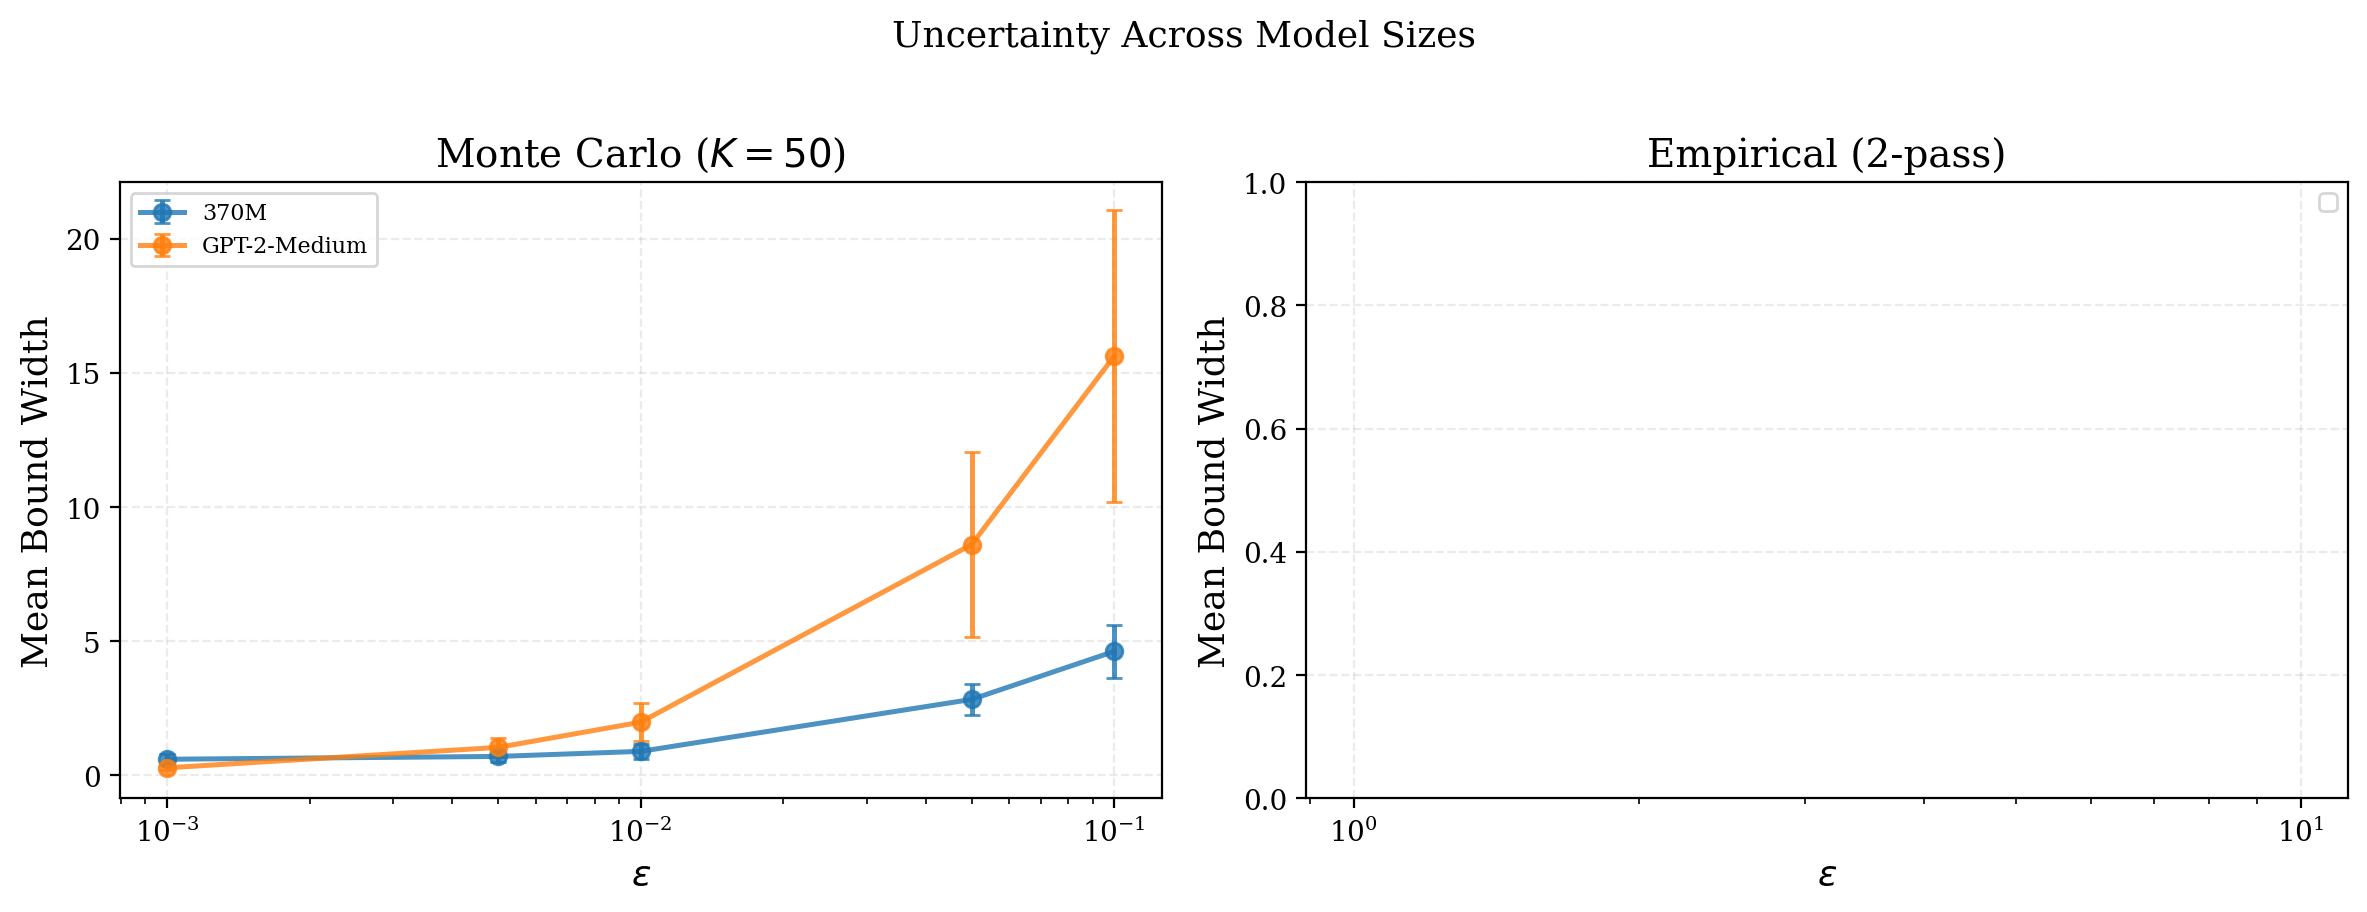
\includegraphics[width=0.85\textwidth]{../results/baseline/plots/baseline_comparison.png}
    \caption{MC empirical bounds ($K{=}50$): MMfreeLM-370M vs.\ GPT-2 Medium (355M). At small $\varepsilon$, both architectures yield comparable bound widths (0.89 vs.\ 1.98 at $\varepsilon{=}0.01$); at $\varepsilon{=}0.1$, MMfreeLM shows substantially lower uncertainty (4.62 vs.\ 15.63). GPT-2 maintains higher top-1 stability despite wider bounds.}
    \label{fig:baseline}
\end{figure}

Figure~\ref{fig:baseline} compares MC bounds for MMfreeLM-370M against GPT-2 Medium. Both models have 24 layers and $\sim$350--370M parameters but differ fundamentally in architecture: MMfreeLM uses ternary BitLinear and gated recurrence, while GPT-2 uses dense MatMul and multi-head self-attention. At $\varepsilon{=}0.01$, GPT-2 Medium shows $\sim$2.2$\times$ wider MC bounds than MMfreeLM (1.98 vs.\ 0.89), and at $\varepsilon{=}0.1$, $\sim$3.4$\times$ wider (15.63 vs.\ 4.62). However, GPT-2 maintains much higher top-1 stability (0.99 vs.\ 0.59 at $\varepsilon{=}0.01$), suggesting its predictions are more robust despite larger logit-magnitude variation. This is partly explained by GPT-2's GELU activation and LayerNorm (which preserves relative logit ordering) versus MMfreeLM's SwiGLU and RMSNorm (which can amplify small embedding changes through multiplicative gating). Overall, the matmul-free architecture's ternary weight discretization does not provide a robustness advantage at the embedding perturbation level.

\section{Discussion}

\subsection{Why ``Addition-Only'' Doesn't Mean ``IBP-Friendly''}

The MMfreeLM paper emphasizes the elimination of MatMul. However, eliminating MatMul does \textbf{not} make the model IBP-friendly:

\begin{enumerate}[nosep]
    \item \textbf{RMSNorm is a division}, not an addition. Division is the most destructive operation for interval arithmetic: output is unbounded when the denominator approaches zero.
    \item \textbf{Multiplicative gating} ($o_t = f_t \odot o_{t-1} + i_t$) creates products of uncertain quantities, growing bounds at each time step. If $f_t$ can approach 1, the recurrence stores and amplifies previous uncertainty.
    \item \textbf{Deep composition}: 24 layers compound any looseness. Even if each individual operation's bound were only 2$\times$ too loose, the compound looseness over 24 layers is $2^{24} \approx 1.7 \times 10^7$.
\end{enumerate}

For IBP to succeed, a model needs a provably small global Lipschitz constant, which typically requires specialized certified training~\cite{gowal2018effectiveness,zhang2019towards}. Neither matmul-free nor standard Transformers have this property out of the box.

\subsection{Limitations}

Our study has several limitations: (1) we perturb embeddings rather than discrete tokens, which is well-defined mathematically but may not correspond to realistic textual perturbations; (2) MC sampling with $K{=}50$ may miss rare extreme outputs accessible to an adversary; (3) the IBP analysis identifies RMSNorm as the bottleneck but does not implement the CROWN fix; (4) the baseline comparison is limited to one model pair (370M vs.\ 355M) and two architectures.

\section{Conclusion}

We presented a study of certified and sampling-based uncertainty quantification for matmul-free language models. Our key findings are:

\begin{enumerate}[nosep]
    \item \textbf{Certified IBP bounds explode} due to RMSNorm (division by a data-dependent quantity) and multiplicative gating in the recurrence. BitLinear (ternary accumulation) layers are well-behaved under IBP; the normalization layers are the sole bottleneck.
    \item \textbf{CROWN / IBP-CROWN} would address this by back-propagating linear bounds rather than forward intervals, potentially providing $\sim$100--1000$\times$ tighter estimates for normalization and recurrent layers.
    \item \textbf{MC sampling provides stable UQ} (bound widths 0.5--10 under $\varepsilon \in [0.001, 0.1]$) and is model-agnostic.
    \item \textbf{Matmul-free and standard Transformers} show comparable perturbation sensitivity, suggesting ternary weight quantization does not fundamentally alter embedding-level robustness.
    \item \textbf{Two-pass corner evaluation} systematically underestimates uncertainty by 2--6$\times$.
\end{enumerate}

All code is open-source and provides a reusable framework for bound propagation analysis of language models.

\begin{thebibliography}{10}

\bibitem{zhu2024scalable}
R.-J.~Zhu, Y.~Zhang, S.~Abreu, E.~Sifferman, T.~Sheaves, Y.~Wang, D.~Richmond, S.~B.~Shrestha, P.~Zhou, and J.~K.~Eshraghian.
\newblock Scalable matmul-free language modeling.
\newblock \emph{arXiv preprint arXiv:2406.02528}, 2024.

\bibitem{gowal2018effectiveness}
S.~Gowal, K.~Dvijotham, R.~Stanforth, R.~Bunel, C.~Qin, J.~Uesato, T.~Mann, and P.~Kohli.
\newblock On the effectiveness of interval bound propagation for training verifiably robust models.
\newblock In \emph{Proceedings of the IEEE International Conference on Computer Vision (ICCV)}, 2019.

\bibitem{zhang2019towards}
H.~Zhang, H.~Chen, C.~Xiao, B.~Li, D.~Boning, and C.-J.~Hsieh.
\newblock Towards Stable and Efficient Training of Verifiably Robust Neural Networks.
\newblock In \emph{ICLR}, 2020.

\bibitem{zhang2018efficient}
H.~Zhang, T.-W.~Weng, P.-Y.~Chen, C.-J.~Hsieh, and L.~Daniel.
\newblock Efficient Neural Network Robustness Certification with General Activation Functions.
\newblock In \emph{NeurIPS}, 2018.

\bibitem{wang2021beta}
S.~Wang, H.~Zhang, K.~Xu, X.~Lin, S.~Jana, C.-J.~Hsieh, and J.~Z.~Kolter.
\newblock Beta-CROWN: Efficient Bound Propagation with Per-Neuron Split Constraints for Neural Network Robustness Verification.
\newblock In \emph{Advances in Neural Information Processing Systems}, 34:29909--29921, 2021.

\bibitem{zhu2023spikegpt}
R.-J.~Zhu, Q.~Zhao, G.~Li, and J.~K.~Eshraghian.
\newblock SpikeGPT: Generative Pre-trained Language Model with Spiking Neural Networks.
\newblock \emph{arXiv preprint arXiv:2302.13939}, 2023.

\end{thebibliography}

\end{document}
